\section[蘇秦以連橫說秦\quad{\small 戰國策 秦策一}]{{\normalsize 戰國策\ 秦策一}\quad \ProperName{蘇秦}以連橫說\ProperName{秦}}
\ProperName{蘇秦}始將連橫說\ProperName{秦惠王},曰:「大王之國,西有\ProperName{巴}、\ProperName{蜀}、\ProperName{漢中}之利,北有\ProperName{胡}貉、\ProperName{代}馬之用,南有\ProperName{巫山}、\ProperName{黔中}之限,東有\ProperName{殽}
\ProperName{函}之固,田肥美,民殷富,戰車萬乘,奮擊百萬,沃野千里,蓄積饒多,地勢形便,此所謂天府,天下之雄國也。以大王之賢,士民之眾,車騎之用,兵法之教,可以幷諸侯,吞天下,稱帝而治。願大王少留意,臣請奏其効。」

\ProperName{秦王}曰:「寡人聞之,毛羽不豐滿者不可以高飛,文章不成者不可以誅罰,道德不厚者不可以使民,政教不順者不可以煩大臣。今先生儼然不遠千里而庭教之,願以異日。」

\ProperName{蘇秦}曰:「臣固疑大王之不能用也。昔者\ProperName{神農}伐\ProperName{補遂},\ProperName{黃帝}伐\ProperName{涿鹿}而禽\ProperName{蚩尤},\ProperName{堯}伐\ProperName{驩兜},\ProperName{舜}伐\ProperName{三苗},\ProperName{禹}伐\ProperName{共工},\ProperName{湯}伐\ProperName{有夏},\ProperName{文王}伐\ProperName{崇},\ProperName{武王}伐\ProperName{紂},\ProperName{齊桓}任戰而霸天下。由此觀之,惡有不戰者乎?古者使車轂擊馳,言語相結,天下爲一。約從連橫,兵革不藏。文士並飭,諸侯亂惑。萬端俱起,不可勝理。科條既備,民多僞態。書策稠濁,百姓不足。上下相愁,民無所聊。明言章理,兵甲愈起。辯言偉服,戰攻不息。繁稱文辭,天下不治。舌敝耳聾,不見成功。行義約信,天下不親。於是及廢文任武,厚養死士,綴甲厲兵,効勝於戰場。夫徒處而致利,安坐而廣地,雖古五帝、三王、五霸,明主賢君,常欲坐而致之,其勢不能,故以戰續之。寬則兩軍相攻,迫則杖戟相橦,然後可建大功。是故兵勝於外,義強於內,威立於上,民服於下。今欲幷天下,凌萬乘,詘敵國,制海內,子元元,臣諸侯,非兵不可。今之嗣主,忽於至道,皆惛於教,亂於治,迷於言,惑於言,沉於辯,溺於辭,以此論之,王固不能行也。」

說\ProperName{秦王}書十上而說不行,黑貂之裘敝,黃金百斤盡。資用乏絕,去\ProperName{秦}而歸。贏縢履蹻,負書擔橐,形容枯槁,面目黧黑,狀有愧色。歸至家,妻不下絍,嫂不爲炊,父母不與言。\ProperName{蘇秦}喟然歎曰:「妻不以我爲夫,嫂不以我爲叔,父母不以我爲子,是皆\ProperName{秦}之罪也!」乃夜發書,陳篋數十,得\BookTitle{太公陰符}之謀。伏而誦之,簡練以爲揣摩。讀書欲睡,引錐自剌其股,血流至足,曰:「安有說人主不能出其金玉錦繡,取卿相之尊者乎?」

期年,揣摩成。曰:「此真可以說當世之君矣。」於是乃摩\ProperName{燕}烏集闕,見說\ProperName{趙王}於華屋之下,抵掌而談。\ProperName{趙王}大悅,封爲\ProperName{武安君},受相印,革車百乘,錦繡千純,白璧百雙,黃金萬鎰,以隨其後。約從散橫,以抑強\ProperName{秦}。故\ProperName{蘇秦}相於\ProperName{趙}而關不通。當此之時,天下之大,萬民之眾,王侯之威,謀臣之權,皆欲決\ProperName{蘇秦}之策。不費斗糧,未煩一兵,未戰一士,未絕一弦,未折一矢,諸侯相親,賢於兄弟。夫賢人在而天下服,一人用而天下從。故曰:「式於政,不式於勇;式於廊廟之內,不式於四境之外。」當\ProperName{秦}之隆,黃金萬鎰爲用,轉轂連騎,炫熿於道。\ProperName{山東}之國,從風而服,使\ProperName{趙}大重。且夫\ProperName{蘇秦}特窮巷掘門、桑戶棬樞之士耳。伏軾撙銜,橫歷天下,庭說諸侯之主,杜左右之口,天下莫之伉。

將說\ProperName{楚王},路過\ProperName{洛陽}。父母聞之,清宮除道,張樂設飲,郊迎三十里。妻側目而視,側耳而聽。嫂蛇行匍伏,四拜自跪而謝。\ProperName{蘇秦}曰:「嫂何前倨而後卑也?」嫂曰:「以季子之位尊而多金。」\ProperName{蘇秦}曰:「嗟乎!貧窮則父母不子,富貴則親戚畏懼。人生世上,勢位富厚,蓋可忽乎哉?」

\section[司馬錯論伐蜀\quad{\small 戰國策 秦策一}]{{\normalsize 戰國策\ 秦策一}\quad \ProperName{司馬錯}論伐\ProperName{蜀}}
\ProperName{司馬錯}與\ProperName{張儀}爭論於\ProperName{秦惠王}前。\ProperName{司馬錯}欲伐\ProperName{蜀},\ProperName{張儀}曰:「不如伐\ProperName{韓}。」王曰:「請聞其說。」

對曰:「親\ProperName{魏}善\ProperName{楚},下兵\ProperName{三川},塞\ProperName{轘轅}、\ProperName{緱氏}之口,當\ProperName{屯留}之道,\ProperName{魏}絕\ProperName{南陽},\ProperName{楚}臨\ProperName{南鄭},\ProperName{秦}攻\ProperName{新城}、\ProperName{宜陽},以臨\ProperName{二周}之郊,誅\ProperName{周主}之罪,侵\ProperName{楚}、\ProperName{魏}之地。\ProperName{周}自知不救,九鼎寶器必出。據九鼎,按圖籍,挾天子以令天下,天下莫敢不聽,此王業也。今夫\ProperName{蜀},西僻之國而戎狄之長也,弊兵\endnote{\BookTitle{觀止}作「名」,下注「作兵」,據\BookTitle{戰國策}校本改。\ProperName{吳師道}\BookTitle{校注}補曰:一本「名」作「兵」。\ProperName{黃丕烈}\BookTitle{札記}:\BookTitle{史記}、\BookTitle{新序}皆作「兵」。\ProperName{范祥雍}\BookTitle{箋證}:\ProperName{鮑}本亦作「兵」,疑一本涉下「名」字而誤。}勞眾不足以成名,得其地不足以爲利。臣聞爭名者於朝,爭利者於市。今\ProperName{三川}、\ProperName{周室},天下之市朝也,而王不爭焉,顧爭於戎狄,去王業遠矣。」

\ProperName{司馬錯}曰:「不然。臣聞之,欲富國者務廣其地,欲強兵者務富其民,欲王者務博其德。三資者備,而王隨之矣。今王之地小民貧,故臣願從事於易。夫\ProperName{蜀},西僻之國也,而戎狄之長也,而有\ProperName{桀}、\ProperName{紂}之亂。以\ProperName{秦}攻之,譬如使豺狼逐羣羊也。取其地足以廣國也,得其財足以富民。繕兵不傷眾,而彼已服矣。故拔一國,而天下不以爲暴;利盡西海,諸侯不以爲貪。是我一舉而名實兩附,而又有禁暴正亂之名。今攻\ProperName{韓}劫天子,劫天子,惡名也,而未必利也,又有不義之名,而攻天下之所不欲,危。臣請謁其故。\ProperName{周},天下之宗室也,\ProperName{韓},\ProperName{周}之與國也。\ProperName{周}自知失九鼎,\ProperName{韓}自知亡三川,則必將二國幷力合謀,以因於\ProperName{齊}、\ProperName{趙},而求解乎\ProperName{楚}、\ProperName{魏}。以鼎與\ProperName{楚},以地與\ProperName{魏},王不能禁。此臣所謂危,不如伐\ProperName{蜀}之完也。」\ProperName{惠王}曰:「善!寡人聽子。」

卒起兵伐\ProperName{蜀},十月取之,遂定\ProperName{蜀}。\ProperName{蜀}主更號爲侯,而使\ProperName{陳莊}相\ProperName{蜀}。\ProperName{蜀}既屬,\ProperName{秦}益強富厚,輕諸侯。

\theendnotes

\section[范雎說秦王\quad{\small 戰國策 秦策三}]{{\normalsize 戰國策\ 秦策三}\quad \ProperName{范雎}說\ProperName{秦王}}
\ProperName{范睢}至,\ProperName{秦王}庭迎\ProperName{范睢},敬執賓主之禮\endnote{「秦王庭迎范睢」下至「敬執賓主之禮」上\BookTitle{觀止}略,\BookTitle{國策}原作:\begin{quotation}\ProperName{秦王}庭迎,謂\ProperName{范睢}曰:「寡人宜以身受令久矣。今者\ProperName{義渠}之事急,寡人日自請太后。今\ProperName{義渠}之事已,寡人乃得以身受命。躬竊閔然不敏,敬執賓主之禮。」\end{quotation}\BookTitle{觀止}「迎」下無「謂」字。\ProperName{范祥雍}\BookTitle{箋證}:\ProperName{鮑}本、\ProperName{吳}本無「謂」字。}。\ProperName{范睢}辭讓。是日見\ProperName{范睢},見者無不變色易容者。

\ProperName{秦王}屏左右,宮中虛無人,\ProperName{秦王}跪而進曰:「先生何以幸教寡人?」\ProperName{范睢}曰:「唯,唯。」有間,\ProperName{秦王}復請,范睢曰:「唯,唯。」若是者三。\ProperName{秦王}跽曰:「先生不幸教寡人乎?」\ProperName{范睢}謝曰:

\begin{quotation}
非敢然也。臣聞始時\ProperName{呂尚}之遇\ProperName{文王}也,身爲漁父而釣於\ProperName{渭陽}之濱耳。若是者交疏也。已一說而立爲太師,載與俱歸者,其言深也。故\ProperName{文王}果收功於\ProperName{呂尚},卒擅天下而身立爲帝王。即使\ProperName{文王}疏\ProperName{呂望}而弗與深言,是\ProperName{周}無天子之德,而\ProperName{文}、\ProperName{武}無與成其王也。今臣,羇旅之臣也,交疏於王,而所願陳者,皆匡君臣之事,處人骨肉之間。願以陳臣之陋忠,而未知王心也,所以王三問而不對者是也。臣非有所畏而不敢言也,知今日言之於前,而明日伏誅於後,然臣弗敢畏也。

大王信行臣之言,死不足以爲臣患,亡不足以爲臣憂,漆身而爲厲,被髮而爲狂,不足以爲臣恥。五帝之聖而死,三王之仁而死,五伯之賢而死,\ProperName{烏獲}之力而死,\ProperName{奔}、\ProperName{育}之勇焉而死。死者,人之所必不免也。處必然之勢,可以少有補於\ProperName{秦},此臣之所大願也,臣何患乎?\ProperName{伍子胥}橐載而出\ProperName{昭關},夜行而晝伏,至於\ProperName{\raisebox{-.45zw}{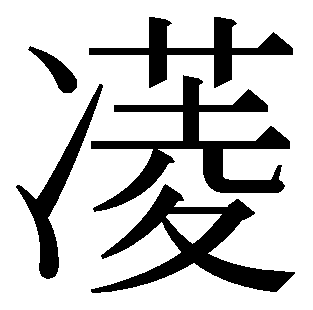
\includegraphics[width=0.9zw,angle=90]{glyphs/u2ff0-u51ab-u83f1.eps}}水}\endnote{\BookTitle{觀止}從\ProperName{鮑}本作「菱夫」,據\BookTitle{戰國策}今校本改。\ProperName{姚}本:\BookTitle{史記}作「\ProperName{陵水}」。},無以餌\endnote{\BookTitle{觀止}作「餬」,據\BookTitle{戰國策}各本改。\ProperName{范祥雍}\BookTitle{箋證}:\BookTitle{范睢傳}「餌」作「餬」;\BookTitle{廣雅}\BookTitle{釋詁}云「餌,食也。」餌、餬義近;\BookTitle{說文}「餬,寄食也。」}其口,坐\endnote{\BookTitle{觀止}作「膝」,據\BookTitle{戰國策}各本改。\ProperName{范祥雍}\BookTitle{箋證}:\BookTitle{范睢傳}作「膝行」,義同。}行蒲服,乞食於\ProperName{吳}巿,卒興\ProperName{吳國},\ProperName{闔廬}爲霸。使臣得進謀如\ProperName{伍子胥},加之以幽囚不復見,是臣說之行也,臣何憂乎?\ProperName{箕子}、\ProperName{接輿},漆身而爲厲,被髮而爲狂,無益於\ProperName{殷}、\ProperName{楚}。使臣得同行於\ProperName{箕子}、\ProperName{接輿},可以補所賢之主,是臣之大榮也,臣又何恥乎?臣之所恐者,獨恐臣死之後,天下見臣盡忠而身蹷也,是以杜口裹足,莫肯即\ProperName{秦}耳\endnote{\BookTitle{觀止}作「因以杜口裹足,莫肯向秦耳」,據\BookTitle{戰國策}各本改。\ProperName{吳師道}\BookTitle{校注}補曰:「即」一作「鄉」。\ProperName{黃丕烈}\BookTitle{札記}:\BookTitle{史記}作「鄉」。\ProperName{范祥雍}\BookTitle{箋證}:按\BookTitle{淮南子}\BookTitle{繆稱訓}\ProperName{高}\BookTitle{注}云「即,就也」「是以」猶「因以」;\BookTitle{范睢傳}作「因以杜口裹足,莫肯鄉\ProperName{秦}耳」。}。足下上畏太后之嚴,下惑姦臣之態,居深宮之中,不離保傅之手,終身闇惑,無與照姦。大者宗廟滅覆,小者身以孤危。此臣之所恐耳。若夫窮辱之事,死亡之患,臣弗敢畏也。臣死而\ProperName{秦}治,賢於生也。
\end{quotation}

\ProperName{秦王}跪曰:「先生是何言也!夫\ProperName{秦國}僻遠,寡人愚不肖,先生乃幸至此,此天以寡人慁先生,而存先王之廟也。寡人得受命於先生,此天所以幸先王而不棄其孤也。先生奈何而言若此!事無大小,上及太后,下至大臣,願先生悉以教寡人,無疑寡人也。」\ProperName{范睢}再拜,\ProperName{秦王}亦再拜。

\theendnotes

\section[鄒忌諷齊王納諫\quad{\small 戰國策 齊策一}]{{\normalsize 戰國策\ 齊策一}\quad \ProperName{鄒忌}諷\ProperName{齊王}納諫}
\ProperName{鄒忌}脩八尺有餘,而形䫉昳麗。朝服衣冠,窺鏡,謂其妻曰:「我孰與城北\ProperName{徐公}美?」其妻曰:「君美甚,\ProperName{徐公}何能及君也。」

城北\ProperName{徐公},\ProperName{齊國}之美麗者也。\ProperName{忌}不自信,而復問其妾曰:「吾孰與\ProperName{徐公}美?」妾曰:「\ProperName{徐公}何能及君也。」

旦日,客從外來,與坐談。問之:「吾與\ProperName{徐公}孰美?」客曰:「\ProperName{徐公}不若君之美也。」

明日,\ProperName{徐公}來,熟視之,自以爲不如。窺鏡而自視,又弗如遠甚。暮寢而思之曰:「吾妻之美我者,私我也。妾之美我者,畏我也。客之美我者,欲有求於我也。」

於是入朝見\ProperName{威王}曰:「臣誠知不如\ProperName{徐公}美。臣之妻私臣,臣之妾畏臣,臣之客欲有求於臣,皆以美於\ProperName{徐公}。今\ProperName{齊}地方千里,百二十城。宮婦左右莫不私王,朝廷之臣莫不畏王,四境之內莫不有求於王。由此觀之,王之蔽甚矣!」

王曰:「善。」乃下令:「羣臣吏民,能面刺寡人之過者,受上賞。上書諫寡人者,受中賞。能謗議於市朝,聞寡人之耳者,受下賞。」令初下,羣臣進諫,門庭若市。數月之後,時時而間進。期年之後,雖欲言,無可進者。\ProperName{燕}、\ProperName{趙}、\ProperName{韓}、\ProperName{魏}聞之,皆朝於\ProperName{齊},此所謂戰勝於朝廷。

\section[顏斶說齊王\quad{\small 戰國策\ 齊策四}]{{\normalsize 戰國策\ 齊策四}\quad \ProperName{顏斶}說\ProperName{齊王}}
\ProperName{齊宣王}見\ProperName{顏斶}曰:「\ProperName{斶}前。」\ProperName{斶}亦曰:「王前。」\ProperName{宣王}不說。左右曰:「王,人君也。\ProperName{斶},人臣也。王曰『\ProperName{斶}前』,\ProperName{斶}亦曰『王前』,可乎?」\ProperName{斶}對曰:「夫\ProperName{斶}前爲慕勢,王前爲趨士,與使\ProperName{斶}爲慕勢,不如使王爲趨士。」

王忿然作色曰:「王者貴乎?士貴乎?」對曰:「士貴耳,王者不貴。」王曰:「有說乎?」\ProperName{斶}曰:「有。昔者\ProperName{秦}攻\ProperName{齊},令曰:『有敢去\ProperName{柳下季}壟五十步而樵採者,死不赦。』令曰:『有能得\ProperName{齊王}頭者,封萬戶侯,賜金千鎰。』由是觀之,生王之頭,曾不若死士之壟也。」\endnote{「死士之壟也」下至「宣王曰」上,\BookTitle{觀止}略。}

\ProperName{宣王}曰:「嗟乎!君子焉可侮哉?寡人自取病耳。願\endnote{「願」上原有「及今聞君子之言,乃今聞細人之行」,\BookTitle{觀止}略。}請受爲弟子,且\ProperName{顏}先生與寡人遊,食必太牢,出必乘車,妻子衣服麗都。」\ProperName{顏斶}辭去曰:「夫玉生於山,制則破焉。非弗寶貴矣,然大璞不完。士生乎鄙野,推選則祿焉。非不得尊遂也,然而形神不全。\ProperName{斶}願得歸,晚食以當肉,安步以當車,無罪以當貴,清淨貞正以自虞。」則再拜而辭去。

君子曰:「\ProperName{斶}知足矣!歸真反璞,則終身不辱。」

\theendnotes

\section[馮煖客孟嘗君\quad {\small 戰國策\ 齊策四}]{{\normalsize 戰國策\ 齊策四}\quad \ProperName{馮煖}客\ProperName{孟嘗君}}
\ProperName{齊}人有\ProperName{馮煖}者,貧乏不能自存,使人屬\ProperName{孟嘗君},願寄食門下。\ProperName{孟嘗君}曰:「客何好?」曰:「客無好也。」曰:「客何能?」曰:「客無能也。」\ProperName{孟嘗君}笑而受之,曰:「諾!」左右以君賤之也,食以草具。

居有頃,倚柱彈其劍,歌曰:「長鋏歸來乎!食無魚!」左右以告。\ProperName{孟嘗君}曰:「食之,比門下之客。」居有頃,復彈其鋏,歌曰:「長鋏歸來乎!出無車!」左右皆笑之,以告。\ProperName{孟嘗君}曰:「爲之駕,比門下之車客。」於是,乘其車,揭其劍,過其友,曰:「\ProperName{孟嘗君}客我!」後有頃,復彈其劍鋏,歌曰:「長鋏歸來乎!無以爲家!」左右皆惡之,以爲貪而不知足。\ProperName{孟嘗君}問:「\ProperName{馮公}有親乎?」對曰:「有老母!」\ProperName{孟嘗君}使人給其食用,無使乏。於是\ProperName{馮煖}不復歌。

後\ProperName{孟嘗君}出記,問門下諸客:「誰習計會,能爲\ProperName{文}收責於\ProperName{薛}者乎?」\ProperName{馮煖}署曰:「能!」\ProperName{孟嘗君}怪之曰:「此誰也?」左右曰:「乃歌夫長鋏歸來者也。」\ProperName{孟嘗君}笑曰:「客果有能也。吾負之,未嘗見也。」請而見之,謝曰:「\ProperName{文}倦於是,憒於憂,而性懧愚,沉於國家之事,開罪於先生。先生不羞,乃有意欲爲收責於\ProperName{薛}乎?」\ProperName{馮煖}曰:「願之!」

於是,約車治裝,載券契而行,辭曰:「責收畢,以何市而反?」\ProperName{孟嘗君}曰:「視吾家所寡有者!」驅而之\ProperName{薛},使吏召諸民當償者,悉來合券。券遍合赴。矯命以責賜諸民,因燒其券,民稱萬歲。長驅到\ProperName{齊},晨而求見。\ProperName{孟嘗君}怪其疾也,衣冠而見之,曰:「責畢收乎?來何疾也!」曰:「收畢矣!」「以何市而反?」\ProperName{馮煖}曰:「君云『視吾家所寡有者』,臣竊計:君宮中積珍寶,狗馬實外廄,美人充下陳。君家所寡有者以義耳!竊以爲君市義。」\ProperName{孟嘗君}曰:「市義奈何?」曰:「今君有區區之\ProperName{薛},不拊愛子其民,因而賈利之。臣竊矯君命,以責賜諸民,因燒其券,民稱萬歲,乃臣所以爲君市義也。」\ProperName{孟嘗君}不說,曰:「諾!先生休矣!」

後期年,\ProperName{齊王}謂\ProperName{孟嘗君}曰:「寡人不敢以先王之臣爲臣!」\ProperName{孟嘗君}就國於\ProperName{薛},未至百里,民扶老攜幼,迎君道中終日。\ProperName{孟嘗君}顧謂\ProperName{馮煖}曰:「先生所爲\ProperName{文}市義者,乃今日見之。」

\ProperName{馮煖}曰:「狡兔有三窟,僅得免其死耳。今君有一窟,未得高枕而臥也,請爲君復鑿二窟。」\ProperName{孟嘗君}予車五十乘,金五百斤,西遊於\ProperName{梁},謂\ProperName{梁王}曰:「\ProperName{齊}放其大臣\ProperName{孟嘗君}於諸侯,諸侯先迎之者富而兵強!」於是,\ProperName{梁王}虛上位,以故相爲上將軍,遣使者黃金千斤,車百乘,往聘\ProperName{孟嘗君}。\ProperName{馮煖}先驅,誡\ProperName{孟嘗君}曰:「千金,重幣也;百乘,顯使也;\ProperName{齊}其聞之矣!」\ProperName{梁}使三反,\ProperName{孟嘗君}固辭不往也。

\ProperName{齊王}聞之,君臣恐懼,遣太傅齎黃金千斤,文車二駟,服劍一,封書謝\ProperName{孟嘗君}曰:「寡人不祥,被於宗廟之崇,沉於諂諛之臣,開罪於君,寡人不足爲也。願君顧先王之宗廟,姑反國,統萬人乎!」\ProperName{馮煖}誡\ProperName{孟嘗君}曰:「願請先王之祭器,立宗廟於\ProperName{薛}。」廟成,還報\ProperName{孟嘗君}曰:「三窟已就,君姑高枕爲樂矣!」

\ProperName{孟嘗君}爲相數十年,無纖介之禍者,\ProperName{馮煖}之計也。

\section[趙威后問齊使\quad{\small 戰國策\ 齊策四}]{{\normalsize 戰國策\ 齊策四}\quad \ProperName{趙威后}問\ProperName{齊}使}
\ProperName{齊王}使使者問\ProperName{趙威后}。書未發,\ProperName{威后}問使者曰:「歲亦無恙耶?民亦無恙耶?王亦無恙耶?」使者不說,曰:「臣奉使使\ProperName{威后},今不問王,而先問歲與民,豈先賤而後尊貴者乎?」\ProperName{威后}曰:「不然。苟無歲何有民?苟無民何有君?故有問,舍本而問末者耶?」

乃進而問之曰:「\ProperName{齊}有處士曰\ProperName{鍾離子},無恙耶?是其爲人也,有糧者亦食,無糧者亦食;有衣者亦衣,無衣者亦衣。是助王養其民者也,何以至今不業也?\ProperName{葉陽子}無恙乎?是其爲人,哀鰥寡,卹孤獨,振困窮,補不足。是助王息其民者也,何以至今不業也?\ProperName{北宮}之女\ProperName{嬰兒子}無恙耶?徹其環瑱,至老不嫁,以養父母。是皆率民而出於孝情者也,胡爲至今不朝也?此二士弗業,一女不朝,何以王\ProperName{齊國},子萬民乎?\ProperName{於陵子仲}尚存乎?是其爲人也,上不臣於王,下不治其家,中不索交諸侯。此率民而出於無用者,何爲至今不殺乎?」

\section[莊辛論幸臣\quad{\small 戰國策\ 楚策四}]{{\normalsize 戰國策\ 楚策四}\quad \ProperName{莊辛}論幸臣}
臣聞鄙語曰:「見兔而顧犬,未爲晚也;亡羊而補牢,未爲遲也。」臣聞昔\ProperName{湯}、\ProperName{武}以百里昌,\ProperName{桀}、\ProperName{紂}以天下亡。今\ProperName{楚國}雖小,絕長續短,猶以數千里,豈特百里哉?王獨不見夫蜻蛉乎?六足四翼,飛翔乎天地之間,俛啄蚉䖟而食之,仰承甘露而飲之。自以爲無患,與人無爭也。不知夫五尺童子,方將調飴膠絲,加己乎四仞之上,而下爲螻蟻食也。夫蜻蛉其小者也,黃雀因是以俯噣白粒,仰棲茂樹,鼓翅奮翼,自以爲無患,與人無爭也。不知夫公子王孫,左挾彈,右攝丸,將加己乎十仞之上,以其類爲招。晝游乎茂樹,夕調乎酸醎,倏忽之間,墜於公子之手。夫雀其小者也,黃鵠因是以。游乎江海,淹乎大沼,府噣鱔鯉,仰嚙䔖衡,奮其六翮,而凌清風,飄搖乎高翔,自以爲無患,與人無爭也。不知夫射者,方將脩其碆盧,治其矰繳,將加己乎百仞之上。被㔋磻,引微繳,折清風而抎矣。故晝游乎江河,夕調乎鼎鼐。

夫黃鵠其小者也,\ProperName{蔡靈侯}之事因是以。南游乎高陂,北陵乎\ProperName{巫山},飲\ProperName{茹谿}流,食\ProperName{湘}波之魚,左抱幼妾,右擁嬖女,與之馳騁乎\ProperName{高蔡}之中,而不以國家爲事。不知夫\ProperName{子發}方受命乎\ProperName{靈王},繫己以朱絲而見之也。\ProperName{蔡靈侯}之事其小者也,君王之事因是以。左\ProperName{州侯},右\ProperName{夏侯},輦從\ProperName{鄢陵君}與\ProperName{壽陵君},飯封祿之粟,而戴方府之金,與之馳騁乎雲夢之中,而不以天下國家爲事。而不知夫\ProperName{穰侯}方受命乎\ProperName{秦王},填\ProperName{黽塞}之內,而投己乎\ProperName{黽塞}之外。

\section[觸讋說趙太后\quad{\small 戰國策\ 趙策四}]{{\normalsize 戰國策\ 趙策四}\quad \ProperName{觸讋}說\ProperName{趙太后}}
\ProperName{趙太后}新用事,\ProperName{秦}急攻之,\ProperName{趙氏}求救於\ProperName{齊}。\ProperName{齊}曰:「必以\ProperName{長安君}爲質,兵乃出。」太后不肯,大臣強諫。太后明謂左右:「有復言令\ProperName{長安君}爲質者,老婦必唾其面。」

左師\ProperName{觸讋}願見,太后盛氣而揖之。入而徐趨,至而自謝曰:「老臣病足,曾不能疾走,不得見久矣。竊自恕,恐太后玉體之有所郄也,故願望見。」太后曰:「老婦恃輦而行。」曰:「日食飲得無衰乎?」曰:「恃鬻耳。」曰:「老臣今者殊不欲食,乃自強步,日三四里,少益嗜食,和於身。」曰:「老婦不能。」太后之色稍解。

左師公曰:「老臣賤息\ProperName{舒祺}最少,不肖,而臣衰,竊愛憐之,願令得補黑衣之數,以衞王宮,沒死以聞。」太后曰:「敬諾。年幾何矣?」對曰:「十五歲矣。雖少,願及未填溝壑而託之。」太后曰:「丈夫亦愛憐其少子乎?」對曰:「甚於婦人。」太后笑曰:「婦人異甚。」對曰:「老臣竊以爲媼之愛\ProperName{燕后},賢於\ProperName{長安君}。」曰:「君過矣!不若\ProperName{長安君}之甚。」左師公曰:「父母之愛子,則爲之計深遠。媼之送\ProperName{燕后}也,持其踵,爲之泣。念悲其遠也,亦哀之矣。已行,非弗思也;祭祀必祝之,祝曰:『必勿使反。』豈非計久長有子孫相繼爲王也哉?」太后曰:「然。」

左師公曰:「今三世以前,至於\ProperName{趙}之爲\ProperName{趙},\ProperName{趙王}之子孫侯者,其繼有在者乎?」曰:「無有。」曰:「微獨\ProperName{趙}諸侯有在者乎?」曰:「老婦不聞也。」「此其近者禍及身,遠者及其子孫。豈人主之子孫,則必不善哉?位尊而無功,奉厚而無勞,而挾重器多也。今媼尊\ProperName{長安}之位,而封以膏腴之地,多予之重器,而不及今令有功於國,一旦山陵崩,\ProperName{長安君}何以自託於\ProperName{趙}?老臣以媼爲\ProperName{長安君}計短也,故以爲其愛不若燕后。」太后曰:「諾。恣君之所使之。」於是爲\ProperName{長安君}約車百乘,質於\ProperName{齊},\ProperName{齊}兵乃出。

\ProperName{子義}聞之曰:「人主之子也,骨肉之親也,猶不能恃無功之尊,無勞之奉,以守金玉之重也,而況人臣乎?」

\section[魯仲連義不帝秦\quad{\small 戰國策\ 趙策三}]{{\normalsize 戰國策\ 趙策三}\quad \ProperName{魯仲連}義不帝\ProperName{秦}}
\ProperName{秦}圍\ProperName{趙}之\ProperName{邯鄲}。\ProperName{魏安釐王}使將軍\ProperName{晉鄙}救\ProperName{趙}。畏\ProperName{秦},止於\ProperName{蕩陰},不進。\ProperName{魏王}使客將軍\ProperName{辛垣衍}間入\ProperName{邯鄲},因\ProperName{平原君}謂\ProperName{趙王}曰:「\ProperName{秦}所以急圍\ProperName{趙}者,前與\ProperName{齊閔王}爭強爲帝,已而復歸帝,以\ProperName{齊}故。今\ProperName{齊閔王}已益弱。方今唯\ProperName{秦}雄天下,此非必貪\ProperName{邯鄲},其意欲求爲帝。\ProperName{趙}誠發使尊\ProperName{秦昭王}爲帝,\ProperName{秦}必喜,罷兵去。」\ProperName{平原君}猶豫未有所決。

此時\ProperName{魯仲連}適游\ProperName{趙},會\ProperName{秦}圍\ProperName{趙}。聞\ProperName{魏}將欲令\ProperName{趙}尊\ProperName{秦}爲帝,乃見\ProperName{平原君}曰:「事將奈何矣?」\ProperName{平原君}曰:「\ProperName{勝}也何敢言事?百萬之眾折於外,今又內圍\ProperName{邯鄲}而不去。\ProperName{魏王}使客將軍\ProperName{辛垣衍}令\ProperName{趙}帝\ProperName{秦}。今其人在是,\ProperName{勝}也何敢言事?」\ProperName{魯連}曰:「始吾以君爲天下之賢公子也,吾乃今然後知君非天下之賢公子也。\ProperName{梁}客\ProperName{辛垣衍}安在?吾請爲君責而歸之。」\ProperName{平原君}曰:「\ProperName{勝}請召而見之於先生。」\ProperName{平原君}遂見\ProperName{辛垣衍}曰:「東國有\ProperName{魯連}先生,其人在此,\ProperName{勝}請爲紹介而見之於將軍。」\ProperName{辛垣衍}曰:「吾聞\ProperName{魯連}先生,\ProperName{齊國}之高士也。\ProperName{衍},人臣也,使事有職。吾不願見\ProperName{魯連}先生也。」\ProperName{平原君}曰:「\ProperName{勝}已泄之矣。」\ProperName{辛垣衍}許諾。

\ProperName{魯連}見\ProperName{辛垣衍}而無言。\ProperName{辛垣衍}曰:「吾視居此圍城之中者,皆有求於\ProperName{平原君}者也。今吾視先生之玉貌,非有求於\ProperName{平原君}者,曷爲久居此圍城之中而不去也?」\ProperName{魯連}曰:「世以\ProperName{鮑焦}無從容而死者,皆非也。今眾人不知,則爲一身。彼\ProperName{秦},棄禮義上首功之國也。權使其士,虜使其民。彼則肆然而爲帝,過而遂正於天下,則\ProperName{連}有赴東海而死耳。吾不忍爲之民也!所爲見將軍者,欲以助\ProperName{趙}也。」\ProperName{辛垣衍}曰:「先生助之奈何?」\ProperName{魯連}曰:「吾將使\ProperName{梁}及\ProperName{燕}助之。\ProperName{齊}、\ProperName{楚}固助之矣。」\ProperName{辛垣衍}曰:「\ProperName{燕}則吾請以從矣。若乃\ProperName{梁},則吾乃\ProperName{梁}人也,先生惡能使\ProperName{梁}助之耶?」\ProperName{魯連}曰:「\ProperName{梁}未睹\ProperName{秦}稱帝之害故也,使\ProperName{梁}睹\ProperName{秦}稱帝之害,則必助\ProperName{趙}矣。」\ProperName{辛垣衍}曰:「\ProperName{秦}稱帝之害將奈何?」\ProperName{魯仲連}曰:「昔\ProperName{齊威王}嘗爲仁義矣,率天下諸侯而朝\ProperName{周}。\ProperName{周}貧且微,諸侯莫朝,而\ProperName{齊}獨朝之。居歲餘,\ProperName{周烈王}崩,諸侯皆弔,\ProperName{齊}後往。\ProperName{周}怒,赴於\ProperName{齊}曰:『天崩地坼,天子下席。東藩之臣\ProperName{田嬰齊}後至,則斮之。』\ProperName{威王}勃然怒曰:『叱嗟,而母婢也。』卒爲天下笑。故生則朝\ProperName{周},死則叱之,誠不忍其求也。彼天子固然,其無足怪。」\ProperName{辛垣衍}曰:「先生獨未見夫僕乎?十人而從一人者,寧力不勝,智不若邪?畏之也。」\ProperName{魯仲連}曰:「然\ProperName{梁}之比於\ProperName{秦}若僕邪?」\ProperName{辛垣衍}曰:「然。」\ProperName{魯仲連}曰:「然則吾將使\ProperName{秦王}烹醢\ProperName{梁王}。」\ProperName{辛垣衍}怏然不說曰:「嘻,亦太甚矣,先生之言也!先生又惡能使\ProperName{秦王}烹醢\ProperName{梁王}?」

\ProperName{魯仲連}曰:「固也,待吾言之。昔者,\ProperName{鬼侯}、\ProperName{鄂侯}、\ProperName{文王},\ProperName{紂}之三公也。\ProperName{鬼侯}有子而好,故入之於\ProperName{紂},\ProperName{紂}以爲惡,醢\ProperName{鬼侯}。\ProperName{鄂侯}爭之急,辨之疾,故脯\ProperName{鄂侯}。文王聞之,喟然而歎,故拘之於\ProperName{牖里}之庫,百日而欲令之死。曷爲與人俱稱帝王,卒就脯醢之地也?\ProperName{齊閔王}將之\ProperName{魯},\ProperName{夷維子}執策而從,謂\ProperName{魯}人曰:『子將何以待吾君?』\ProperName{魯}人曰:『吾將以十太牢待子之君。』\ProperName{夷維子}曰:『子安取禮而來待吾君?彼吾君者,天子也。天子巡狩,諸侯避舍,納於筦鍵,攝衽抱几,視膳於堂下,天子已食,退而聽朝也。』\ProperName{魯}人投其籥,不果納。不得入於\ProperName{魯},將之\ProperName{薛},假塗於\ProperName{鄒}。當是時,\ProperName{鄒君}死,\ProperName{閔王}欲入弔。\ProperName{夷維子}謂\ProperName{鄒}之孤曰:『天子弔,主人必將倍殯柩,設北面於南方,然後天子南面弔也。』\ProperName{鄒}之羣臣曰:『必若此,吾將伏劍而死。』故不敢入於\ProperName{鄒}。\ProperName{鄒}、\ProperName{魯}之臣,生則不得事養,死則不得飯含。然且欲行天子之禮於\ProperName{鄒}、\ProperName{魯}之臣,不果納。今\ProperName{秦}萬乘之國,\ProperName{梁}亦萬乘之國。俱據萬乘之國,交有稱王之名,賭其一戰而勝,欲從而帝之,是使\ProperName{三晉}之大臣不如\ProperName{鄒}、\ProperName{魯}之僕妾也。且\ProperName{秦}無已而帝,則且變易諸侯之大臣。彼將奪其所謂不肖,而予其所謂賢;奪其所憎,而與其所愛。彼又將使其子女讒妾爲諸侯妃姬,處\ProperName{梁}之宮,\ProperName{梁王}安得晏然而已乎?而將軍又何以得故寵乎?」

於是,\ProperName{辛垣衍}起,再拜謝曰:「始以先生爲庸人,吾乃今日而知先生爲天下之士也。吾請去,不敢復言帝\ProperName{秦}。」\ProperName{秦}將聞之,爲郤軍五十里。

適會\ProperName{公子無忌}奪\ProperName{晉鄙}軍以救\ProperName{趙}擊\ProperName{秦},\ProperName{秦}軍引而去。

於是\ProperName{平原君}欲封\ProperName{魯仲連}。\ProperName{魯仲連}辭讓者三,終不肯受。\ProperName{平原君}乃置酒,酒酣,起前以千金爲\ProperName{魯連}壽。\ProperName{魯連}笑曰:「所貴於天下之士者,爲人排患、釋難、解紛亂而無所取也。即有所取者,是商賈之人也,\ProperName{仲連}不忍爲也。」遂辭\ProperName{平原君}而去,終身不復見。

\section[魯共公擇言\quad{\small 戰國策\ 魏策二}]{{\normalsize 戰國策\ 魏策二}\quad \ProperName{魯共公}擇言}
\ProperName{梁王}\ProperName{魏嬰}觴諸侯於\ProperName{范臺},酒酣,請\ProperName{魯君}舉觴。\ProperName{魯君}興,避席擇言曰:「昔者帝女令\ProperName{儀狄}作酒而美,進之\ProperName{禹},\ProperName{禹}飲而甘之,遂疏\ProperName{儀狄},絕旨酒,曰:『後世必有以酒亡其國者。』\ProperName{齊桓公}夜半不嗛,\ProperName{易牙}乃煎敖燔炙和調五味而進之,\ProperName{桓公}食之而飽,至旦不覺,曰:『後世必有以味亡其國者。』\ProperName{晉文公}得\ProperName{南之威},三日不聽朝,遂推\ProperName{南之威}而遠之,曰:『後世必有以色亡其國者。』\ProperName{楚王}登\ProperName{強臺}而望\ProperName{崩山},左江而右湖,以臨\ProperName{彷徨},其樂忘死,遂盟\ProperName{強臺}而弗登,曰:『後世必有以高臺陂池亡其國者。』今主君之尊,\ProperName{儀狄}之酒也;主君之味,\ProperName{易牙}之調也;左\ProperName{白台}而右\ProperName{閭須},\ProperName{南威}之美也;前\ProperName{夾林}而後\ProperName{蘭臺},\ProperName{強臺}之樂也。有一於此,足以亡其國。今主君兼此四者,可無戒與?」\ProperName{梁王}稱善相屬。

\section[唐雎說信陵君\quad{\small 戰國策\ 魏策四}]{{\normalsize 戰國策\ 魏策四}\quad \ProperName{唐雎}說\ProperName{信陵君}}
\ProperName{信陵君}殺\ProperName{晉鄙},救\ProperName{邯鄲},破\ProperName{秦}人,存\ProperName{趙國},\ProperName{趙王}自郊迎。

\ProperName{唐雎}謂\ProperName{信陵君}曰:「臣聞之曰,事有不可知者,有不可不知者;有不可忘者,有不可不忘者。」

\ProperName{信陵君}曰:「何謂也?」

對曰:「人之憎我也,不可不知也;吾\endnote{\BookTitle{觀止}作「我」,據\BookTitle{戰國策}各本改。}憎人也,不可得而知也。人之有德於我也,不可忘也;吾有德於人也,不可不忘也。今君殺\ProperName{晉鄙},救\ProperName{邯鄲},破\ProperName{秦}人,存\ProperName{趙國},此大德也。今\ProperName{趙王}自郊迎,卒然見\ProperName{趙王},臣願君之忘之也。」

\ProperName{信陵君}曰:「\ProperName{無忌}謹受教。」

\theendnotes

\section[唐雎不辱使命\quad{\small 戰國策\ 魏策四}]{{\normalsize 戰國策\ 魏策四}\quad \ProperName{唐雎}不辱使命}
\ProperName{秦王}使人謂\ProperName{安陵君}曰:「寡人欲以五百里之地易\ProperName{安陵},\ProperName{安陵君}其許寡人?」\ProperName{安陵君}曰:「大王加惠,以大易小,甚善。雖然,受地於先王,願終守之,弗敢易。」\ProperName{秦王}不說。\ProperName{安陵君}因使\ProperName{唐雎}使於\ProperName{秦}。

\ProperName{秦王}謂\ProperName{唐雎}曰:「寡人以五百里之地易\ProperName{安陵},\ProperName{安陵君}不聽寡人,何也?且\ProperName{秦}滅\ProperName{韓}亡\ProperName{魏},而君以五十里之地存者,以君爲長者,故不錯意也。今吾以十倍之地,請廣於君,而君逆寡人者,輕寡人與?」\ProperName{唐雎}對曰:「否,非若是也。\ProperName{安陵君}受地於先王而守之,雖千里不敢易也,豈直五百里哉?」

\ProperName{秦王}怫然怒,謂\ProperName{唐雎}曰:「公亦嘗聞天子之怒乎?」\ProperName{唐雎}對曰:「臣未嘗聞也。」\ProperName{秦王}曰:「天子之怒,伏屍百萬,流血千里。」\ProperName{唐雎}曰:「大王嘗聞布衣之怒乎?」\ProperName{秦王}曰:「布衣之怒,亦免冠徒跣,以頭搶地耳。」\ProperName{唐雎}曰:「此庸夫之怒也,非士之怒也。夫\ProperName{專諸}之刺\ProperName{王僚}也,彗星襲月;\ProperName{聶政}之刺\ProperName{韓傀}也,白虹貫日;\ProperName{要離}之刺\ProperName{慶忌}也,倉\endnote{\BookTitle{觀止}作「蒼」,據\BookTitle{戰國策}各本改。\ProperName{吳師道}\BookTitle{校注}補曰:「倉」即「蒼」。}鷹擊於殿上。此三子者,皆布衣之士也,懷怒未發,休祲降於天,與臣而將四矣。若士必怒,伏屍二人,流血五步,天下縞素,今日是也。」挺劍而起。

\ProperName{秦王}色撓,長跪而謝之曰:「先生坐,何至於此,寡人諭矣。夫\ProperName{韓}、\ProperName{魏}滅亡,而\ProperName{安陵}以五十里之地存者,徒以有先生也。」

\theendnotes

\section[樂毅報燕王書\quad{\small 戰國策\ 燕策二}]{{\normalsize 戰國策\ 燕策二}\quad \ProperName{樂毅}報\ProperName{燕王}書}
\ProperName{昌國君}\ProperName{樂毅}爲\ProperName{燕昭王}合五國之兵而攻\ProperName{齊},下七十餘城,盡郡縣之以屬燕。三城未下,而\ProperName{燕昭王}死。\ProperName{惠王}即位,用\ProperName{齊}人反間,疑\ProperName{樂毅},而使\ProperName{騎劫}代之將。\ProperName{樂毅}奔\ProperName{趙},\ProperName{趙}封以爲\ProperName{望諸君}。\ProperName{齊}\ProperName{田單}詐\ProperName{騎劫},卒敗\ProperName{燕}軍,復收七十餘城以復\ProperName{齊}。\ProperName{燕王}悔,懼\ProperName{趙}用\ProperName{樂毅}承\ProperName{燕}之弊以伐\ProperName{燕}。

\ProperName{燕王}乃使人讓\ProperName{樂毅},且謝之曰:「先王舉國而委將軍,將軍爲\ProperName{燕}破\ProperName{齊},報先王之讎,天下莫不振動,寡人豈敢一日而忘將軍之功哉!會先王棄羣臣,寡人新即位,左右誤寡人。寡人之使\ProperName{騎劫}代將軍,爲將軍久暴露於外,故召將軍且休計事。將軍過聽,以與寡人有隙,遂捐\ProperName{燕}而歸\ProperName{趙}。將軍自爲計則可矣,而亦何以報先王之所以遇將軍之意乎?」

\ProperName{望諸君}乃使人獻書報\ProperName{燕王}曰:

\begin{quotation}
臣不佞,不能奉承先王之教,以順左右之心,恐抵斧質之罪,以傷先王之明,而又害於足下之義,故遁逃奔\ProperName{趙}。自負以不肖之罪,故不敢爲辭說。今王使使者數之罪,臣恐侍御者之不察先王之所以畜幸臣之理,而又不白於臣之所以事先王之心,故敢以書對。

臣聞賢聖之君,不以祿私其親,功多者授之;不以官隨其愛,能當者處之。故察能而授官者,成功之君也;論行而結交者,立名之士也。臣以所學者觀之,先王之舉錯,有高世之心,故假節於\ProperName{魏王},而以身得察於\ProperName{燕}。先王過舉,擢之乎賓客之中,而立之乎羣臣之上,不謀於父兄,而使臣爲亞卿。臣自以爲奉令承教,可以幸無罪矣,故受命而不辭。

先王命之曰:「我有積怨深怒於\ProperName{齊},不量輕弱,而欲以\ProperName{齊}爲事。」臣對曰:「夫\ProperName{齊},霸國之餘教也,而驟勝之遺事也,閑於兵甲\endnote{\BookTitle{觀止}倒作「甲兵」,據\BookTitle{戰國策}各本改。},習於戰攻。王若欲攻之,則必舉天下而圖之。舉天下而圖之,莫徑於結\ProperName{趙}矣。且又\ProperName{淮北}、\ProperName{宋}地,\ProperName{楚}\ProperName{魏}之所同願也。\ProperName{趙}若許,約\ProperName{楚}、\ProperName{魏},\ProperName{宋}盡力,四國攻之,\ProperName{齊}可大破也。」先王曰:「善。」臣乃口受令,具符節,南使臣於\ProperName{趙}。顧反命,起兵隨而攻\ProperName{齊}。以天之道,先王之靈,\ProperName{河北}之地,隨先王舉而有之於\ProperName{濟上}。\ProperName{濟上}之軍,奉令擊\ProperName{齊},大勝之。輕卒銳兵,長驅至國。\ProperName{齊王}逃遁走\ProperName{莒},僅以身免。珠玉財寶,車甲珍器,盡收入\ProperName{燕}。大呂陳於\ProperName{元英},故鼎反於\ProperName{曆室},\ProperName{齊}器設於\ProperName{寧臺}。\ProperName{薊丘}之植,植於\ProperName{汶}篁。自五伯以來,功未有及先王者也。先王以爲順于其志,以臣爲不頓命,故裂地而封之,使之得比乎小國諸侯。臣不佞,自以爲奉令承教,可以幸無罪矣,故受命而弗辭。

臣聞賢明之君,功立而不廢,故著於\BookTitle{春秋};蚤知之士,名成而不毀,故稱於後世。若先王之報怨雪恥,夷萬乘之強國,收八百歲之蓄積,及至棄羣臣之日,遺令詔後嗣之餘義,執政任事之臣,所以能循法令,順庶孽者,施及萌隸,皆可以教於後世。

臣聞善作者,不必善成;善始者,不必善終。昔者\ProperName{伍子胥}說聽乎\ProperName{闔閭},故\ProperName{吳王}遠跡至於\ProperName{郢}。\ProperName{夫差}弗是也,賜之鴟夷而浮之江。故\ProperName{吳王}\ProperName{夫差}不悟先論之可以立功,故沉\ProperName{子胥}而弗悔。\ProperName{子胥}不蚤見主之不同量,故入江而不改。夫免身全功,以明先王之跡者,臣之上計也。離毀辱之非,墮先王之名者,臣之所大恐也。臨不測之罪,以幸爲利者,義之所不敢出也。

臣聞古之君子,交絕不出惡聲;忠臣之去也,不潔其名。臣雖不佞,數奉教於君子矣。恐侍御者之親左右之說,而不察疏遠之行也。故敢以書報,唯君之留意焉。
\end{quotation}
\vspace{-1em}
\theendnotes

\section[李斯諫逐客書\quad{\small 秦文}]{{\normalsize 秦文}\quad \ProperName{李斯}諫逐客書}
\ProperName{秦}宗室大臣皆言\ProperName{秦王}曰:「諸侯人來事\ProperName{秦}者,大抵爲其主遊閒於\ProperName{秦}耳,請一切逐客。」\ProperName{李斯}議亦在逐中。\ProperName{斯}乃上書曰:

\begin{quotation}
臣聞吏議逐客,竊以爲過矣。昔\ProperName{穆公}求士,西取\ProperName{由余}於\ProperName{戎},東得\ProperName{百里奚}於\ProperName{宛},迎\ProperName{蹇叔}於\ProperName{宋},求\ProperName{丕豹}、\ProperName{公孫支}於\ProperName{晉}。此五子者,不產於\ProperName{秦},而\ProperName{穆公}用之,幷國二十,遂霸\ProperName{西戎}。\ProperName{孝公}用\ProperName{商鞅}之法,移風易俗,民以殷盛,國以富彊,百姓樂用,諸侯親服,獲\ProperName{楚}、\ProperName{魏}之師,舉地千里,至今治彊。\ProperName{惠王}用\ProperName{張儀}之計,拔\ProperName{三川}之地,西幷\ProperName{巴}、\ProperName{蜀},北收\ProperName{上郡},南取\ProperName{漢中}。包九夷,制\ProperName{鄢}、\ProperName{郢},東據\ProperName{成皋}\endnote{\BookTitle{觀止}作「城皋」,據\BookTitle{史記}本改。}之險,割膏腴之壤,遂散六國之從,使之西面事\ProperName{秦},功施到今。\ProperName{昭王}得\ProperName{范雎},廢\ProperName{穰侯},逐\ProperName{華陽},彊公室,杜私門,蠶食諸侯,使\ProperName{秦}成帝業。此四君者,皆以客之功。由此觀之,客何負於\ProperName{秦}哉!向使四君卻客而不內,疏士而不與,是使國無富利之實,而\ProperName{秦}無彊大之名也。

今陛下致\ProperName{昆山}之玉,有\ProperName{隨}、\ProperName{和}之寶,垂明月之珠,服太阿之劍,乘纖離之馬,建翠鳳之旗,樹靈鼉之鼓。此數寶者,\ProperName{秦}不生一焉,而陛下說之,何也?必\ProperName{秦國}之所生然後可,則是夜光之璧不飾朝廷,犀象之器不爲玩好,\ProperName{鄭}、\ProperName{衞}\endnote{\BookTitle{觀止}作「魏」,據\BookTitle{史記}本改。}之女不充後宮,而駿良\endnote{\BookTitle{觀止}作「馬」,\BookTitle{崇古文訣}、\BookTitle{冊府元龜}同,據\BookTitle{史記}本改。}駃騠不實外廄,\ProperName{江南}金錫不爲用,\ProperName{西蜀}丹青不爲采。所以飾後宮充下陳娛心意說耳目者,必出於\ProperName{秦}然後可,則是\ProperName{宛}珠之簪,傅璣之珥,阿縞之衣,錦繡之飾不進於前,而隨俗雅化佳冶窈窕\ProperName{趙}女不立於側也。夫擊甕叩缶,彈箏搏髀,而歌呼嗚嗚快耳目者,真\ProperName{秦}之聲也;\BookTitle{鄭}、\BookTitle{衞}、\BookTitle{桑間}、\BookTitle{韶}、\BookTitle{虞}、\BookTitle{武}、\BookTitle{象}者,異國之樂也。今棄擊甕叩缶\endnote{\BookTitle{觀止}「擊甕」下無「叩缶」二字,據\BookTitle{史記}補。\BookTitle{文選考異}:\ProperName{袁}本、\ProperName{茶陵}本無「叩缶」二字。}而就\BookTitle{鄭}\BookTitle{衞},退彈箏而取\BookTitle{韶}\BookTitle{虞},若是者何也?快意當前,適觀而已矣。今取人則不然,不問可否,不論曲直,非\ProperName{秦}者去,爲客者逐,然則是所重者在乎色樂珠玉,而所輕者在乎人民也。此非所以跨海內,致諸侯之術也。

臣聞地廣者粟多,國大者人眾,兵彊則士勇。是以\ProperName{太山}不讓士壤,故能成其大;河海不擇細流,故能就其深;王者不卻眾庶,故能明其德。是以地無四方,民無異國,四時充美,鬼神降福。此\ProperName{五帝}、\ProperName{三王}之所以無敵也。今乃棄黔首以資敵國,卻賓客以業諸侯,使天下之士退而不敢西向,裹足不入\ProperName{秦},此所謂「藉寇兵而齎盜糧者」也。

夫物不產於\ProperName{秦},可寶者多;士不產於\ProperName{秦},而願忠者眾。今逐客以資敵國,損民以益讎,內自虛而外樹怨於諸侯,求國無危\endnote{\BookTitle{觀止}「國」下有「之」字,據\BookTitle{史記}本刪。},不可得也。
\end{quotation}

\ProperName{秦王}乃除逐客之令,復\ProperName{李斯}官。

\theendnotes

\section[卜居\quad{\small 楚辭}]{{\normalsize 楚辭}\quad 卜居}
\ProperName{屈原}既放,三年不得復見,竭智盡忠,而蔽鄣於讒,心煩慮亂,不知所從。乃往見太卜\ProperName{鄭詹尹}曰:「余有所疑,願因先生決之。」\ProperName{詹尹}乃端策拂龜曰:「君將何以教之?」\ProperName{屈原}曰:「吾寧悃悃款款,朴以忠乎?將送往勞來,斯無窮乎?寧誅鋤草茅,以力耕乎?將遊大人,以成名乎?寧正言不諱,以危身乎?將從俗富貴,以媮生乎?寧超然高舉,以保真乎?將哫訾慄斯,喔咿嚅唲,以事婦人乎?寧廉潔正直,以自清乎?將突梯滑稽,如脂如韋,以絜楹乎?寧昂昂若千里之駒乎?將氾氾若水中之鳧?與波上下,偷以全吾軀乎?寧與騏驥亢軛乎?將隨駑馬之迹乎?寧與黃鵠比翼乎?將與雞鶩爭食乎?此孰吉孰凶?何去何從?世溷濁而不清:蟬翼爲重,千鈞爲輕;黃鐘毀棄,瓦釜雷鳴;讒人高張,賢士無名。吁嗟默默兮,誰知吾之廉貞!」

\ProperName{詹尹}乃釋策而謝曰:「夫尺有所短,寸有所長;物有所不足,智有所不明,數有所不逮,神有所不通。用君之心,行君之意。龜策誠不能知此事。」

\section[宋玉對楚王問\quad{\small 楚辭}]{{\normalsize 楚辭}\quad \ProperName{宋玉}對\ProperName{楚王}問}
\ProperName{楚襄王}問於\ProperName{宋玉}曰:「先生其有遺行與?何士民眾庶不譽之甚也!」

\ProperName{宋玉}對曰:「唯,然,有之。願大王寬其罪,使得畢其辭。客有歌於\ProperName{郢}中者,其始曰\BookTitle{下里}、\BookTitle{巴人},國中屬而和者數千人;其爲\BookTitle{陽阿}、\BookTitle{薤露},國中屬而和者數百人;其爲\BookTitle{陽春}、\BookTitle{白雪},國中屬而和者不過數十人;引商刻羽,雜以流徵,國中屬而和者不過數人而已。是其曲彌高,其和彌寡。故鳥有鳳而魚有鯤,鳳凰上擊九千里,絕雲霓,負蒼天,足亂浮雲,翱翔乎杳冥之上。夫藩籬之鷃,豈能與之料天地之高哉?鯤魚朝發\ProperName{崑崙}之墟,暴鬐於\ProperName{碣石},暮宿於\ProperName{孟諸}。夫尺澤之鯢,豈能與之量江海之大哉?故非獨鳥有鳳而魚有鯤也,士亦有之。夫聖人瑰意琦行,超然獨處;世俗之民,又安知臣之所爲哉?」

% Proofed 12 July  2022
% Ref. 
% 戰國策, 上海古籍, 1985
% 文選, 上海古籍, 1986
% 點校本史記, 中華書局, 1959
% 楚辭集注, 上海古籍, 1979